\documentclass{tufte-handout}
\pagenumbering{arabic}
\usepackage{amsmath}
\usepackage[pdftex]{graphicx}
\usepackage{color}
\usepackage{enumitem}
\usepackage{natbib}
\usepackage{comment}
\usepackage{bm}
\usepackage{mdwlist}

% The following package makes prettier tables.  We're all about the bling!
\usepackage{booktabs}

% The units package provides nice, non-stacked fractions and better spacing
% for units.
\usepackage{units}

\newcommand{\angstrom}{\text{\normalfont\AA}}

% The fancyvrb package lets us customize the formatting of verbatim
% environments.  We use a slightly smaller font.
\usepackage{fancyvrb}
\fvset{fontsize=\normalsize}

% Small sections of multiple columns
\usepackage{multicol}

\usepackage{hyperref}
\hypersetup{
    colorlinks=true,       % false: boxed links; true: colored links
    linkcolor=red,       % color of internal links
    citecolor=red,        % color of links to bibliography
    filecolor=magenta,      % color of file links
    urlcolor=blue           % color of external links
}

\newcommand{\cs}{${}^{137}_{\ 55}{\rm Cs}$ }
\newcommand{\ba}{${}^{137}_{\ 56}{\rm Ba }$}
\newcommand{\bam}{${}^{137}_{\ 56}{\rm Ba^* }$}

%\pagestyle{myheadings}
%\markright{Fall~2016\hspace{1.9in}Mechanics Lab}


%\documentclass[12pt]{aastex}
%\usepackage{graphicx,mdwlist,longtable,url}
%\usepackage[final]{pdfpages}
%
%\usepackage[title,titletoc,toc]{appendix}
%\usepackage{longtable}
%
%% left-justify the section headings and make them bigger
%\usepackage{titlesec}
%\newcommand*{\justifyheading}{\raggedright}
%\titleformat*{\section}{\Large\bfseries}
%\titleformat*{\subsection}{\large\bfseries}
%
%\renewcommand{\bottomfraction}{0.9}
%
%\setlength{\parindent}{0.cm}
%\setlength{\parskip}{0.3cm}
%\setlength{\topmargin}{-1.3cm}
%\setlength{\textheight}{9in}
%\setlength{\evensidemargin}{0cm}
%\setlength{\textwidth}{6.46in}
%\setlength{\oddsidemargin}{0in}
%
%\pagestyle{myheadings}
%\markright{Fall~2016\hspace{1.9in}Mechanics Lab}
%
%% these make the longtables span the width of \textwidth
%\setlength\LTleft{0pt}
%\setlength\LTright{0pt}



\begin{document}
{\LARGE {\em 
\noindent Modern Physics---PHYS~220
\vspace{0.5mm}

\noindent Fall 2023
\vspace{3mm}
}}


{\LARGE {\em \noindent Lab: $e/m$ with Teltron Deflection Tube}}

\large{\noindent Josh Diamond,  John Cummings, George Hassel, Mark Rosenberry, \& Matt Bellis}


\vspace{0.5cm}
\noindent{\bf \LARGE Week 2}\\
\vspace{0.5cm}

\section{Overview}

In this lab you will measure the deflection of an electron beam by electric and
magnetic fields infer the charge-to-mass ratio $e/m$ for the electron.

\section{Theory}

A charged particle with charge $q$ in an electric field $\vec{E}$
experiences a force given by:
\begin{equation}
\vec{F}_E = q \vec{E}
\end{equation}

\noindent If the particle moves with velocity $\vec{v}$ in a magnetic field
$\vec{B}$, the force on the particle is:
\begin{equation}
\label{lorentz}
\vec{F}_B = q \vec{v} \times \vec{B}
\end{equation}

For an electron, the charge $q = -e$, where $e = 1.6 \times 10^{-19}$~Coulomb is
the fundamental unit of positive charge. The mass $m$ of the electron is $m =
9.11 \times 10^{-31}$~kg.

In this experiment, the electrons are accelerated through a voltage
$V_a$ before entering the region containing the fields
under study. Due to the accelerating voltage, the electrons acquire a
kinetic energy equal to the loss of potential energy $eV_a$, {\em i.e.}:
\begin{equation}
\label{energy}
\frac{1}{2} mv^{2} = eV_a
\end{equation}

\subsection{Deflection In a Magnetic Field}

We shall study the motion of an electron in a uniform magnetic field.  Newton's
second law states that $\vec{F} = m\vec{a}$. Let us apply this relation to a
beam of electrons traveling perpendicular to the magnetic field at speed
$v$. Since the magnetic force on an electron is perpendicular to its velocity,
the electron speed stays constant and the electron travels in a circular path.

The magnitude of the magnetic force in Eq. 2 then simplifies to
$F_{B }= evB$, and the acceleration of the electron in its
circular path becomes $a = v^{2}/r$, where $r$ is the radius
of the circle. Substituting into Newton's second law,
we get:


\begin{align}
\label{newton}
F &= ma \nonumber \\
evB &= m\frac{v^{2}}{r}
\end{align}

Equations \ref{energy} and \ref{newton} may be combined to eliminate the electron speed $v$, and
solved for the charge to mass ratio, $e/m$. One then finds:

\begin{equation}
\label{eom}
\boxed{ e/m = \frac{2V_a}{B^2r^2} }
\end{equation}

In this experiment, the magnetic field is produced by a pair of identical coils
carrying the same current. The coils are separated with spacing equal to the
coil radius.\sidenote{A pair of such coils are known as \textbf{Helmholtz
    coils}, and produce a rather uniform magnetic field in the vicinity of the
  midpoint between the coils along the coil axis.} It can be shown that the
magnetic field in this region is given approximately by:
\begin{equation}
\label{helmholtz}
\boxed{ B=\frac{8 \mu_0 N I}{a \sqrt{125}} }
\end{equation}
\noindent where $\mu_0 = 4\pi \times 10^{-7} $ Tm/A, $N$ is the number of turns
in each coil, $I$ is the current through the coils, and $a$ is the radius of
each coil.\sidenote{For the Teltron Helmholtz coils, $N = 320$ and $a = 6.8$ cm
  $= 0.068$~m.}

Using the Teltron tube, the electron beam is accelerated horizontally into the
region where the magnetic field is present. Using the coordinate grid built into
the apparatus, one can determine points through which the electron beam
passes. If the circle formed by the electron path passes horizontally through
the origin, and also passes through the point (x,y), one can easily show that
the radius of the circle is given by:\sidenote{See Figure~\ref{circularpath}.}
\begin{equation}
\label{circle}
\boxed{ r=\frac{x^2+y^2}{2y} }
\end{equation}

\begin{figure}
\begin{center}
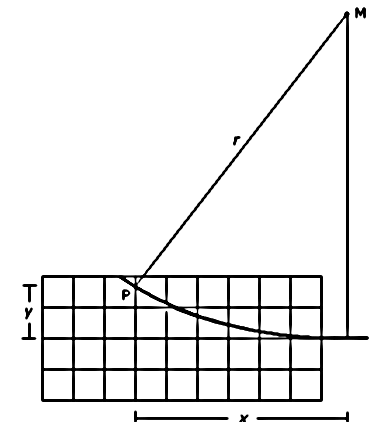
\includegraphics[width=2in]{../images/radius.png}
\caption{Geometry of electron's circular path through magnetic field.}
\label{circularpath}
\end{center}
\end{figure}

\section{Preliminary Questions}

\begin{enumerate}
\item Obtain Eq.~\ref{eom} from Eqs.~\ref{energy} and \ref{newton}.
\item Derive Eq.~\ref{circle}.
\item Using the given numerical data, write Eq.~\ref{helmholtz} in the form $B = CI$,
where $C$ is a numerical constant that you can evaluate from Eq.~\ref{helmholtz}.
What are the units of $B$ and $I$? 
\end{enumerate}

\section{Apparatus}

See Figure~\ref{tubepic} to reference the relevant features of the $e/m$ deflection tube:

\begin{enumerate}
\item Fluorescent screen
\item Lower deflection plate (not used)
\item Boss with 4 mm plug for connecting deflection plate (not used)
\item Electron gun
\item 4 mm sockets for connecting heater supply and cathode
\item 4 mm plug for connecting anode (accelerating voltage)
\item Upper deflection plate (not used)
\end{enumerate}

\begin{figure}
\begin{center}
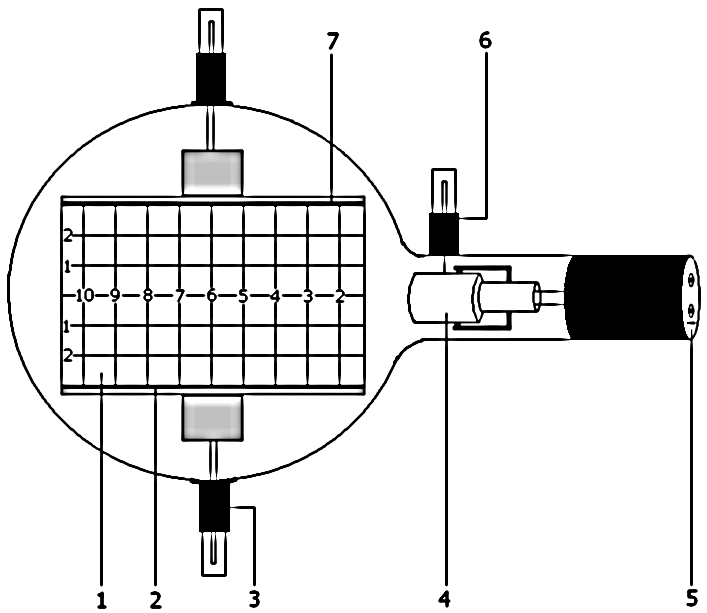
\includegraphics[width=4in]{../images/teltron525.png} 
\caption{Location of terminals on Teltron 525 deflection tube.}
\label{tubepic}
\end{center}
\end{figure}



As shown in Fig.~\ref{tubewiring2}, the tube contains four terminals for electrical
connections, two for the AC voltage (6 V) that serves to heat the
filament and two for the DC accelerating voltage $V_a$.
 Note that the two larger receptacles on the base of the tube connect
to AC terminals of the power supply.  The smaller receptacle is to be
connected to the negative DC terminal.  The positive DC voltage
terminal is connected to the plug pointing perpendicular to the tube
axis located near the electron gun.
%The power supply has 6.3 volt terminals for the filament heating current and high voltage terminals for the accelerating voltage.  
The Helmholtz coils have a separate power supply, and should be connected in a series loop containing the power supply, coils, and ammeter. The full circuit diagram is shown in Figure~\ref{tubewiring}.

\begin{figure}
\begin{center}
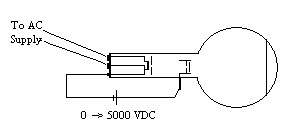
\includegraphics[width=3.0929in,height=1.3543in]{../images/ediffraction-img1.png}
\caption{Schematic diagram of electron diffraction tube.}
\label{tubewiring2}
\end{center}
\end{figure}


\begin{figure}
\begin{center}
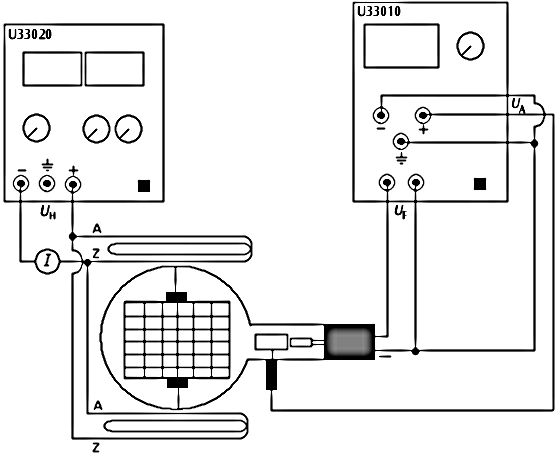
\includegraphics[width=4in]{../images/wiring.png} 
\caption{Wiring schematic for Teltron 525 deflection tube.}
\label{tubewiring}
\end{center}
\end{figure}


\section{Procedure}

\textbf{CAUTION}\textbf{: \ High voltages are used in this experiment.
Always slide the high voltage control on the power supply to its lowest
setting before making any changes in the circuit. Have the instructor
check your circuit when you change it before increasing the
voltage.}

\begin{enumerate}
\item Connect the circuit as shown, omitting the electric
field deflection connection,  and with no current running through the
Helmholtz coils. Gradually increase the accelerating voltage until you
see the path of the electron beam on the calibrated fluorescent
screen.



\item Place a bar magnet near the tube to illustrate deflection of the beam. Try various orientations of the bar
magnet. Which gives the largest deflection of the beam?


\item Place the bar magnet perpendicular to the beam with the north pole
nearest to the tube. Using the right hand rule, predict the direction
of the magnetic force on the electrons. Compare to the observed
deflection of the beam.


\item Turn on the Helmholtz coil circuit. Try varying the
magnetic field (by varying the Helmholtz coil current). What is the
effect on the radius of curvature of the electron beam path?

For fixed magnetic field, try varying the accelerating voltage. What is
the effect on the electron beam path radius of curvature?


\item For an accelerating voltage of 2500 volts, adjust the magnetic field
  current so that the beam passes through a known point.  For instance, the far
  corner of the calibrated region has coordinates $(x,y) = (10~\rm{cm},
  2.5~\rm{cm})$ . Record the current.


\item Repeat step 5 for larger voltages, incrementing in
steps of 500 volts up to a maximum of 4500 volts.
\end{enumerate}

\section{Analysis}

\begin{enumerate}
\item Explain the results obtained in Procedure steps 1-4 qualitatively
in terms of the appropriate relationships. Hint: for 2 \& 3, consider
the magnetic force law, Eq.~\ref{lorentz}; for step 4, Eq.~\ref{eom} will be helpful.

\item For each set of $V$ and $B$ data taken in Procedure step 5, compute $e/m$
for the electron. Use SI units throughout.

\item Find the mean value of $e/m$ and the uncertainty (standard deviation of
the mean). Compare your results (including the uncertainty) to
$e/m$ as obtained from standard values of $e$ and $m$.
\end{enumerate}

\section{Uncertainty Analysis}

To determine the uncertainty on the electron-to-mass ratio, $e/m$, look again at
Eqs.~\ref{eom}, \ref{helmholtz}, and \ref{circle}. The expression for $e/m$
depends on $V_a$, $B$, and $r$; $r$, in turn, depends on $x$ and $y$, while $B$
depends on $I$.
%One way to find the uncertainty is with addition in quadrature:
%\begin{equation}
%\sigma(e/m) = \sqrt{ \left(\frac{\sigma_{Va}}{V_a}\right)^2 +
%  \left(\frac{2\sigma_B}{B}\right)^2 + \left(\frac{2\sigma_r}{r}\right)^2 },
%\end{equation}
%\noindent where we define $\sigma_B$ and $\sigma_r$ below.
The total uncertainty, $\sigma(e/m)$, therefore, is:
\begin{equation}
\sigma(e/m) = \sqrt{ 
  \left(\frac{\partial(e/m)}{\partial V_a} \sigma_{Va}\right)^2 + 
  \left(\frac{\partial(e/m)}{\partial B} \sigma_B\right)^2 + 
  \left(\frac{\partial(e/m)}{\partial r} \sigma_r\right)^2 },
\label{eq:sigma_eom}
\end{equation}
\noindent where $\sigma_{Va}$, $\sigma_B$, and $\sigma_r$ are the uncertainties
on $V_a$, $B$, and $r$, respectively. 

Although this equation may appear intimidating, you can attack it in parts:
\begin{itemize}
  \item First, derive an expression for $\partial(e/m)/\partial V_a$ and
    multiply by $\sigma_{Va}$ to get the uncertainty due to the accelerating
    voltage.
  \item Next, derive an expression for $\partial(e/m)/\partial B$. Here,
    although you don't have an uncertainty in $B$, you can easily show that
    $\sigma_B = C\sigma_I$, where $C$ is the constant determined in the lab, and
    $\sigma_I$ is the measured uncertainty in the current. Substitute these
    results into your expression to get the uncertainty on $e/m$ due to the
    $B$-field.
  \item Finally, first derive an expression for $\partial(e/m)/\partial r$ and
    use the following result (which you could also derive yourself!):
    \begin{equation}
      \sigma_r = \sqrt{ \left(\frac{x}{y}\sigma_x\right)^2 +
        \left(\frac{y^2-x^2}{2y^2} \sigma_y\right)^2 }.
    \end{equation}
\end{itemize}

Determine if any of the terms in Eq.~\ref{eq:sigma_eom} are negligibly small
compared to the others and, if so, you can ignore them from your final
calculations. 

Finally, you can also compare the standard deviation of the mean of $e/m$ you
measure from multiple trials against the formal uncertainty you determine using
the procedure above. Are they different and, if so, why?


\section{References}
\begin{itemize}
\item Thornton and Rex, Modern Physics, $3^{\rm rd}$ ed., pp. 85-89
\item Equipment instructions: Teltron 525 Deflection Tube
\item Tipler and Llewellan, Modern Physics,$5^{\rm th}$ ed., pp. 116-118
\end{itemize}


\end{document}

 
